\chapter{Replacements for t-tests and ANOVA}
ANOVA is a common procedure in classical statistics, and is related to the
simpler idea of a t-test. These classical tests were designed for particular
kinds of problems, and in this chapter we will study similar problems but
solve them from a Bayesian point of view.
We will also use these examples to discuss some issues about the choice
of prior distributions when there are more than a few parameters. When there
are only a few parameters it is usually safe to assign a vague, wide prior
to describe your initial uncertainty (unless, of course, you have more
information than that). In higher dimensions, problems can arise if you do
this. One way of getting around these problems is to use a
{\it hierarchical model}.

\section{A T-Test Example}
This example is based on one given in a 1976 article by physicist E. T. Jaynes,
called ``Confidence Intervals vs. Bayesian Intervals''. This is a very strongly
worded paper and might be an interesting read for
those who are interested in the battle between frequentist and Bayesian statistics
when the latter was making its comeback in the second half of the 20th century.
It's also where I got the crazy confidence interval example from.

Two manufacturers, $1$ and $2$, both make ``widgets'', and we are interested
in figuring out which manufacturer makes the best widgets (on average), as
measured by their lifetime. To determine this, we obtain 9 widgets from
manufacturer $1$ and 4 widgets from manufacturer $2$, and measure their
lifetimes, in days. The results are given below:
\begin{eqnarray}
x^1 &=& \{41.26, 35.81, 36.01, 43.59, 37.50, 52.70, 42.43, 32.52, 56.20\}\\
x^2 &=& \{54.97, 47.07, 57.12, 40.84\}
\end{eqnarray}
These measurements can be summarised by the means and standard deviations, which
are $42 \pm 7.48$ for group $1$ and $50 \pm 6.48$ for group $2$.
The question is: given this data, is there evidence that one of the manufacturers
is better than the other, and if so, by how much?
In classical statistics the standard procedure for this situation would be a
two sample $t$0-test. However, before we do anything I'd like you to consider
the numbers and use your intuition: what do {\it you} think about what the
evidence says?

An underlying assumption of a classical $t$-test is that the data are normally
distributed around the mean values for each group\footnote{Strictly speaking,
it's the probability distribution for the data given the parameters
that is normal, the data may or may not look normally distributed.}.
We may as well adopt this
assumption for our Bayesian model. If we call the group 1
data points $\{x^1_1, x^1_2, ..., x^1_{N_1}\}$ and the group 2 data points
$\{x^2_1, x^2_2, ..., x^2_{N_1}\}$, then the likelihood is:
\begin{eqnarray}
x^1_i &\sim& \mathcal{N}\left(\mu_1, \sigma^2\right)\nonumber\\
x^2_i &\sim& \mathcal{N}\left(\mu_2, \sigma^2\right)\label{eq:ttest_likelihood}
\end{eqnarray}
Where all the data points are independent given the parameters. Note the assumption that
the two groups have the same underlying (``population'') standard deviation $\sigma$. This is a popular
assumption in this kind of analysis but it is not necessarily well justified!
We will build our Bayesian models using this assumption, but it is not that
difficult to relax it if you want to. You could just include multiple
$\sigma$ parameters in the model,
just like how we will include the multiple $\mu$ parameters.

Instead of just one model for this situation, we will study three different
versions. Each model will have the same likelihood
as given above in Equation~\ref{eq:ttest_likelihood}, and the same prior
for $\sigma$. However, the models will all have different priors for $\mu_1$
and $\mu_2$.
We will be able to see that the choice of prior does
influence the results (of course), but in ways that make sense. Which of these
models is more appropriate in a practical situation would depend on the exact
situation. There is no ``one size fits all'' model.

\subsection{Likelihood}
To implement our model in JAGS, we can begin by specifying the likelihood
part like so:

\begin{minted}[mathescape,
               numbersep=5pt,
               gobble=0,
               frame=single,
               framesep=2mm, fontsize=\small]{r}
# Sampling distribution/likelihood
for(i in 1:N1)
{
  x1[i] ~ dnorm(mu1, 1/sigma^2)
}
for(i in 1:N2)
{
  x2[i] ~ dnorm(mu2, 1/sigma^2)
}
\end{minted}
We have called our data arrays {\tt x1} and {\tt x2}, and we have also
assumed that the sample sizes {\tt N1} and {\tt N2} are defined, so our
{\tt data} list will need to be consistent with these choices. The parameters
we will be estimating are {\tt mu1}, {\tt mu2}, and {\tt sigma}, so we will
need to specify prior distributions for them. In the following sections, we'll
use the same prior for {\tt sigma}, so we may as well specify that now.
Let's use a log-uniform prior where $\sigma$ is between $e^{-10}$ and
$e^{10}$.

\begin{minted}[mathescape,
               numbersep=5pt,
               gobble=0,
               frame=single,
               framesep=2mm, fontsize=\small]{r}
# Prior for sigma
log_sigma ~ dunif(-10, 10)
sigma <- exp(log_sigma)
\end{minted}

\subsection{Prior 1: Very Vague}
The last missing ingredients to finish the JAGS model are the priors for
{\tt mu1} and {\tt mu2}. For our first model, let's be really naive and assign
super-wide uniform priors.

\begin{minted}[mathescape,
               numbersep=5pt,
               gobble=0,
               frame=single,
               framesep=2mm, fontsize=\small]{r}
# Prior 1: Very Vague
mu1 ~ dnorm(0, 1/1000^2)
mu2 ~ dnorm(0, 1/1000^2)
\end{minted}

At first glance, this might seem like a fairly reasonable thing to do. In many
problems, it doesn't make much difference if we just use vague priors and get
on with the calculation (as opposed to thinking really hard about the prior,
and what is actually known about the parameters).

However, this prior has a number of properties that suggest it might not be
quite right: firstly, what is the probability that $\mu_1 = \mu_2$?
In classical t-tests, the whole point is to test the hypothesis that
the two ``population means'' (parameters) are equal. However, our prior
actually implies that the probability they are equal is 0! Therefore, no matter
what data we get, the posterior probability of $\mu_1 = \mu_2$ will always be
zero.

\subsection{Prior 2: They might be equal!}
The problem with Prior 1 is that we may think $\mu_1$ might exactly equal
$\mu_2$, and Prior 1 doesn't allow for this. So here's another way we might
set up the prior. We'll start by defining the prior for $\mu_1$ as we did
before. Then, when we consider $\mu_2$, we need a way of giving it a
50\% probability of equalling $\mu_1$, and if not, then it should have
a ``bi-exponential'' distribution centered around $\mu_1$.
Here is our solution. Read it carefully and make sure you understand what this
prior does.

\begin{minted}[mathescape,
               numbersep=5pt,
               gobble=0,
               frame=single,
               framesep=2mm, fontsize=\small]{r}
# First mean
mu1 ~ dnorm(0, 1/1000^2)

# Prior for difference, mu2 - mu1
u ~ dunif(-1, 1)

# Length of exponential prior given difference != 0
L <- 5
size_of_difference <- step(u)*(-L*log(1 - u))

# To make the difference positive or negative
C ~ dbin(0.5, 1)
difference <- (2*C - 1)*size_of_difference

# Second mean
mu2 <- mu1 + difference
\end{minted}

\subsection{Prior 3: Alright, they're not equal, but they might be {\it close}}
Prior 2 is also a little bit strange, if you think about it. If we're comparing
these two manufacturers of widgets, why would we think it is possible that the
two manufacturers are {\tt exactly} equal? Maybe we just think the parameters
$\mu_1$ and $\mu_2$ are likely to be {\it similar} in value.
In other words, we shouldn't worry so much about the
prior probablity of $\mu_1 = \mu_2$, but we should at least make sure there's
a moderate prior probability that $\mu_1 \approx \mu_2$.

One way we could do this is by applying a normal prior to both $\mu_1$ and
$\mu_2$ with some mean (let's call it the ``grand mean'')
and some standard deviation (let's call it the ``diversity'').
That way, $\mu_1$ and
$\mu_2$ would both be likely to be somewhere around the grand mean, and
they would likely be different by roughly the size of the diversity.
The challenge now seems to be the choice of appropriate values for the grand
mean and the diversity. Fortunately, we don't actually have to! What we can
do instead is apply priors for them instead.

This is our first example of a {\it hierarchical model}. In a hierarchical
model, instead of directly assigning priors to our parameters, we imagine that
we knew the values of some other parameters (called ``hyperparameters''), and
assign our prior for the parameters {\it given} the hyperparameters. Then we
assign a prior for they hyperparameters as well, to complete the model.

\begin{minted}[mathescape,
               numbersep=5pt,
               gobble=0,
               frame=single,
               framesep=2mm, fontsize=\small]{r}
# Hierarchical prior for the means
# Hyperparameters
grand_mean ~ dnorm(0, 1/1000^2)
log_diversity ~ dunif(-10, 10)
diversity <- exp(log_diversity)

# Prior for the parameters given the hyperparameters
mu1 ~ dnorm(grand_mean, 1/diversity^2)
mu2 ~ dnorm(grand_mean, 1/diversity^2)
\end{minted}

Samples (obtained using JAGS) of the three priors are shown in
Figure~\ref{fig:ttest1}.
\begin{figure}[!ht]
\begin{center}
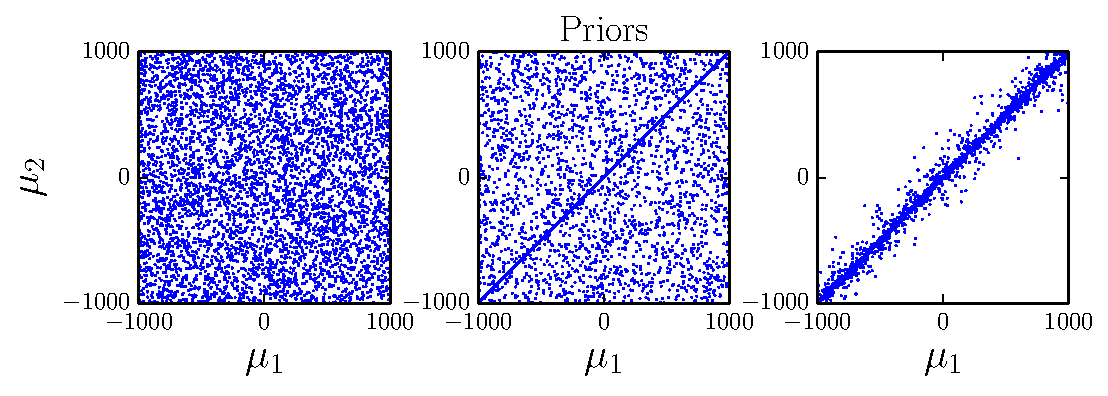
\includegraphics[scale=0.8]{Figures/ttest1.pdf}
\caption{\it The three different priors we are trying for our Bayesian
equivalent of a t-test. The first prior simply asserts a large amount of
prior ignorance about the value of the two parameters $\mu_1$ and $\mu_2$.
The second is similar but applies 50\% probability to the proposition
$\mu_1 = \mu_2$. The third prior does not allow the two parameters to be
exactly equal, but enhances the probability that they are quite similar
in value.\label{fig:ttest1}}
\end{center}
\end{figure}

The posteriors are shown in Figure~\ref{fig:ttest2}.
The inferences are different, as you would expect, and that's entirely down
to the choice of the prior. Any summaries we make will therefore depend on
which prior we want to use.
\begin{figure}[!ht]
\begin{center}
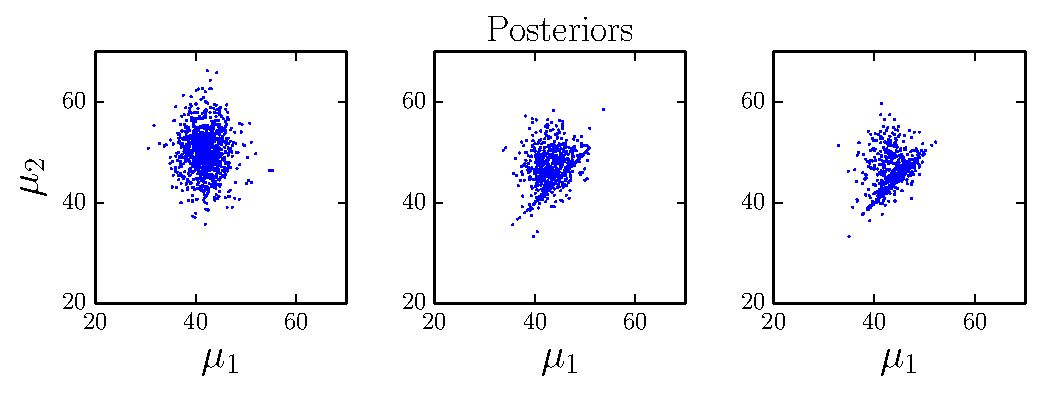
\includegraphics[scale=0.8]{Figures/ttest2.pdf}
\caption{\it The posterior distributions, given the widget data,
based on the three different priors for $\mu_1$ and $\mu_2$.\label{fig:ttest2}}
\end{center}
\end{figure}

The original question was whether manufacturer two was better, equal, or worse
than manufacturer one. We can answer that question by calculating the
posterior probabilities of $\mu_1 = \mu_2$, $\mu_1 < \mu_2$, and
$\mu_1 > \mu_2$. The results are shown in Table~\ref{tab:ttest_results}.

\begin{table}
\begin{center}
{\bf Prior Probabilities}:\\
\vspace{0.3cm}
\begin{tabular}{|l|c|c|c|}
\hline
Prior	&	$\mu_1 < \mu_2$	& $\mu_1 = \mu_2$	& $\mu_1 > \mu_2$\\
\hline
1 	&	0.5		&	0		&	0.5\\
2 	&	0.25		&	0.5		&	0.25\\
3 	&	0.5		&	0		&	0.5\\
\hline
\end{tabular}\\
\vspace{0.5cm}
{\bf Posterior Probabilities}:\\
\vspace{0.3cm}
\begin{tabular}{|l|c|c|c|}
\hline
Prior	&	$\mu_1 < \mu_2$	& $\mu_1 = \mu_2$	& $\mu_1 > \mu_2$\\
\hline
1 	&	0.945		&	0		&	0.055\\
2 	&	0.491		&	0.430		&	0.079\\
3 	&	0.629		&	0		&	0.372\\
\hline
\end{tabular}
\caption{\it Prior and posterior probabilities for three different hypotheses about
the two manufacturers, based on the models with the three different priors.
As you can see, the conclusions are quite sensitive to the choice of prior in
this case.
\label{tab:ttest_results}}
\end{center}
\end{table}

Remember that Prior 1 did not assign any probability to the possibility of the
two parameters being equal. Therefore, no possible evidence can increase
make the posterior probability nonzero. However, according to this model, there
is quite strong evidence that $\mu_1 < \mu_2$, as the probability changed from
0.5 to 0.946.

Prior 2 did allow the two parameters to be equal, and if we use Prior 2, we
seem to have found very weak evidence that they are not in fact equal. The probability
decreased from 0.5 to 0.424. According to Prior 2, if $\mu_1 \neq \mu_2$, then
$\mu_1 < \mu_2$ is the next most likely scenario. However, Prior 2 has an issue
associated with it. Our prior says that if $\mu_2$ is not equal to $\mu_1$, then
it is likely to be close to $\mu_1$. Exactly how close we expect it to be is
set by the variable {\tt L} in the model.
If we were to make {\tt L} very large, then the data would go from weak evidence
against $\mu_1 = \mu_2$ to strong evidence for it! Why does this happen? Well,
if we increased {\tt L}, the prior probability that $\mu_2$ and $\mu_1$ are
close given that they're different is decreased. Then, the hypothesis that
the $\mu$s are different does not predict our data as well, since our data
looks like the $\mu$s are close together. Since it doesn't predict the data as
well as before, its posterior probability will be lower.
 Some people think this sensitivity to the prior is a
danger of Bayesian inference (if you want, you can do a web search for the
``Jeffreys-Lindley paradox''),
but it is behaving logically: the wider we make
the prior, the lower we make the prior probability that $\mu_1$ and $\mu_2$
are close but not equal, giving the model no choice but to believe that they're
equal. If the results are sensitive to the prior, that's important, and you
should think about the logic of the problem to understand why.

Prior 3 seems like it's what we might want in general. It's often silly to think
two parameters might be {\it exactly} equal. What we really think is that there
is a difference, and it might be very small, or moderate or large.

\section{One Way Anova}
One-way ANOVA can be considered as a generalisation of a t-test to more than
two groups. The question is usually phrased as a test of the hypothesis that
the group means are the same, versus the alternative that there is some difference.
As we saw in the Bayesian ``t-test'', it is possible (using clever tricks) to
make a model that has some prior probability that the group means are equal.
However, this gets more tricky with multiple groups. Therefore we will build our
one-way ANOVA model in a similar way to the ``hierarchical model'' version of the
t-test model. There will be one other major difference, but it is a difference
in the way the model is coded, not a conceptual difference.

In the t-test section our data set was composed of measurements in two groups
and our data list contained two vectors of measurements, called {\tt x1} and
{\tt x2}. The sampling distribution/likelihood part of our JAGS model also
needed two {\tt for} loops, one for each group.
If we have many groups (in the following example we will have four),
it can get awkward having to write all those loops. Therefore, when we develop
our ``one-way ANOVA'' model, we will format the data differently by putting
all measurements into a single vector {\tt x}. To make this work, we'll need
an extra vector in the dataset, which tells us which group each data point
belongs to.

We'll use an example dataset on the masses of starlings (a type of bird).
The masses of some starlings were measured at four locations. We are interested
in the differences between the locations. How similar are they in terms of the
average weight of starlings? Are they basically the same, radically different,
or something in between? A boxplot of the data is shown in
Figure~\ref{fig:starling}, which seems to show substantial differences between
the locations. However, only ten starlings were measured at each location, so
we can't be absolutely sure of this, and our goal is to investigate how
sure we should be.

To solve this problem in a Bayesian way, we will treat it as a parameter
estimation problem with four $\mu$ parameters, one for each of the locations.
We will also need at least one parameter describing the standard deviation
of the starling masses at each location. For convenience we'll assume that's
the same across all locations, but it is straightforward to relax this
assumption later.

\begin{figure}[!ht]
\begin{center}
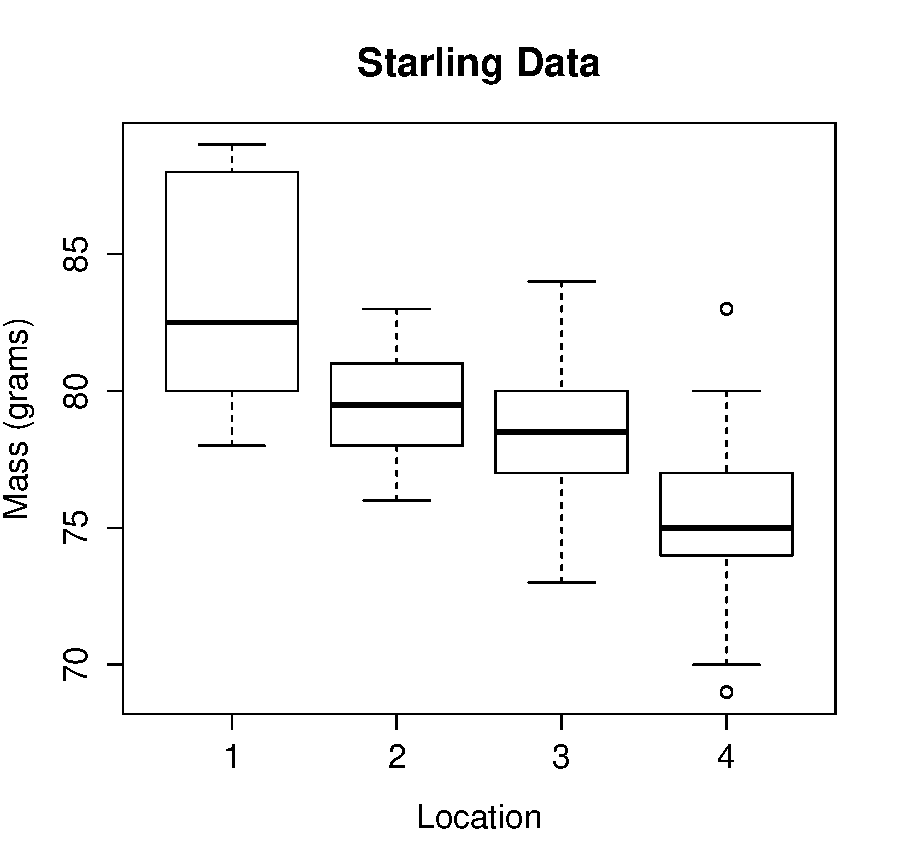
\includegraphics[scale=0.6]{Figures/starling.pdf}
\caption{\it The masses of starlings as measured at four different locations.
It seems as though the mean mass varies somewhat according to the location, and
our results will tell us how plausible this is.
\label{fig:starling}}
\end{center}
\end{figure}


\subsection{Hierarchical Model}
Our ``one-way ANOVA'' model is very much the same as our final ``t-test'' model,
except for the format of the dataset.
The main advantage of this model is that it generalises to more than two groups
in a very straightforward way; we no longer need to write separate for loops
for each group. As with the third ``t-test'' model, we are not seriously
considering the hypothesis that all of the group means (i.e. the $\mu$
parameters) are exactly equal, but we are allowing them to be quite close
together, or quite distinct in value, by using the hierarchical model
structure with the {\tt diversity} parameter.

\begin{minted}[mathescape,
               numbersep=5pt,
               gobble=0,
               frame=single,
               framesep=2mm, fontsize=\small]{r}
model
{
    # Log-uniform prior for the scatter
    log_sigma ~ dunif(-10, 10)
    sigma <- exp(log_sigma)

    # Hierarchical prior for the means
    # Hyperparameters
    grand_mean ~ dnorm(0, 1/1000^2)
    log_diversity ~ dunif(-10, 10)
    diversity <- exp(log_diversity)

    # Parameters
    for(i in 1:N)
    {
      mu[i] ~ dnorm(grand_mean, 1/diversity^2)
    }

    # Sampling distribution/likelihood
    for(i in 1:N)
    {
        x[i] ~ dnorm(mu[group[i]], 1/sigma^2)
    }
}
\end{minted}

After running this model on the starling data, we can plot any results we
wish. In Figure~\ref{fig:trace_starlings2}, I have plotted a trace plot of
$\mu_1$, the parameter for the mean weight of starlings at location 1. This
is a healthy trace plot, although there is a strange feature near iteration
1000 which we will discuss in the next section. Figure~\ref{fig:diversity}
shows the posterior distribution for the {\tt log\_diversity} hyperparameter,
which quantifies how different the groups really are. Our prior for this
parameter was U(-10, 10), and the posterior peaks at around 1.5, which
corresponds to {\tt diversity} $\approx$ 4.5, although there is a fair bit of
uncertainty. Notice also the long tail of the posterior on the left hand side.
Although we never allowed the $\mu$s to be exactly the same, we did allow them
to be close (and this corresponds to the diversity being low). The fact that
some posterior samples landed between -10 and 0 suggests there is a small
probability that the differences between groups are very small, despite the
fact that the data doesn't look that way.

\begin{figure}[!ht]
\begin{center}
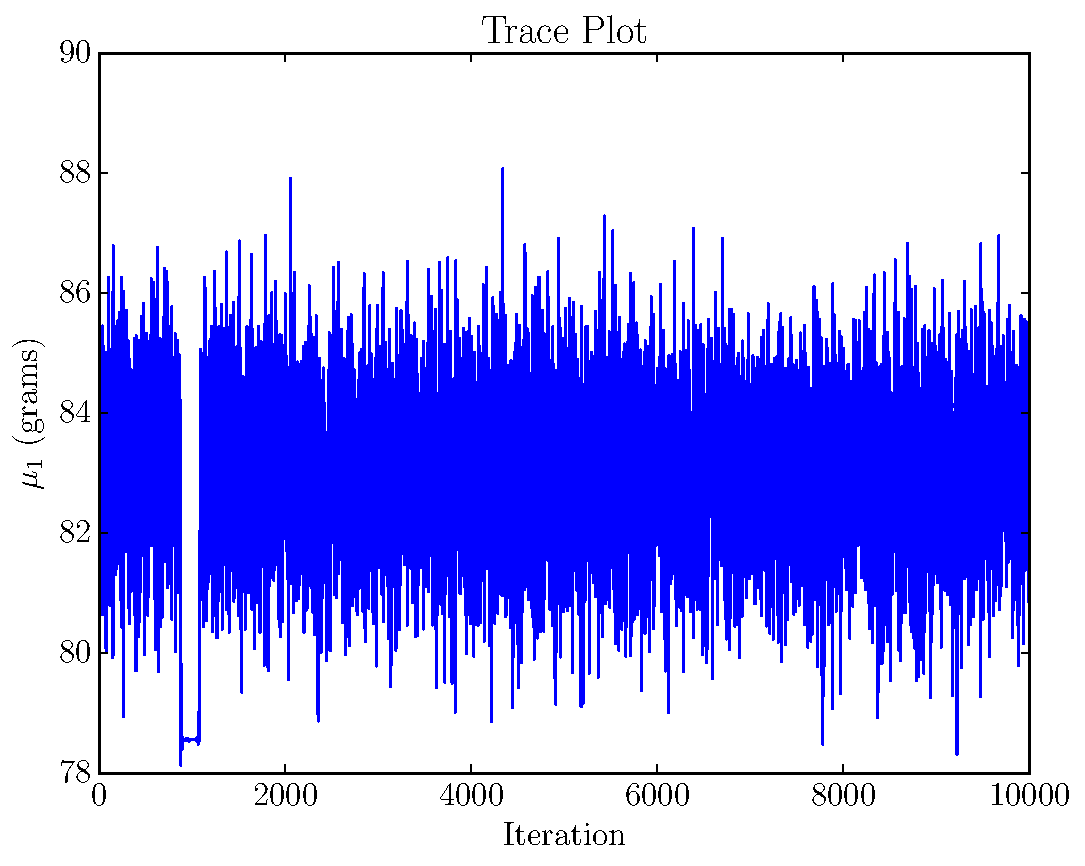
\includegraphics[scale=0.6]{Figures/trace_starlings.pdf}
\caption{\it A trace plot of $\mu_1$ from a JAGS run on the starling data. Things
appear to be mixing well, except for an odd feature near iteration 1000.
\label{fig:trace_starlings2}}
\end{center}
\end{figure}

\begin{figure}[!ht]
\begin{center}
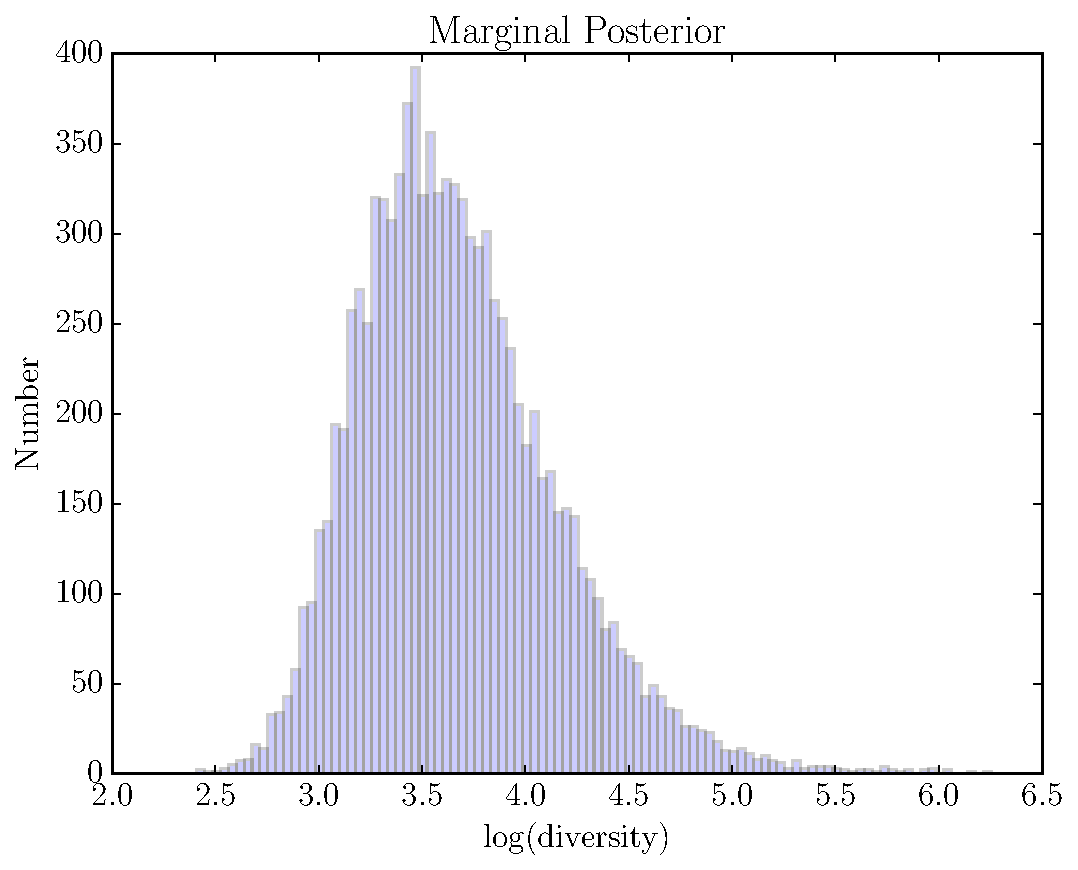
\includegraphics[scale=0.6]{Figures/diversity.pdf}
\caption{\it The posterior distribution for {\tt log\_diversity}.\label{fig:diversity}}
\end{center}
\end{figure}

As usual, we can use our posterior samples to calculate the posterior
probability of any hypothesis that we can think of based on the parameters.
Here are a couple of interesting examples:
\begin{minted}[mathescape,
               numbersep=5pt,
               gobble=0,
               frame=single,
               framesep=2mm, fontsize=\small]{r}
# Is mu2 really greater than mu3?
> mean(results\$mu[,2] > results\$mu[,3])
[1] 0.672
# Is the diversity really less than 1 (log diversity less than 0)?
> mean(results\$diversity < 0)
[1] 0.0272
\end{minted}

\subsection{MCMC Efficiency}
The hierarchical ``one-way ANOVA'' model given above works, but a quick look
at the trace plot suggests the mixing (how easily the MCMC algorithm is
able to move around) isn't very good. In some models, it makes sense to
consider the {\it parameterisation} of the model. There are actually different
ways to implement exactly the same model assumptions, but in a way that helps
the efficiency of the MCMC sampling.

Let's look at a small subset of the above model: just the hierarchical prior
for the $\mu$s. Here it is:

\begin{minted}[mathescape,
               numbersep=5pt,
               gobble=0,
               frame=single,
               framesep=2mm, fontsize=\small]{r}
# Hierarchical prior for the means
# Hyperparameters
grand_mean ~ dnorm(0, 1/1000^2)
log_diversity ~ dunif(-10, 10)
diversity <- exp(log_diversity)

# Parameters
for(i in 1:N)
{
  mu[i] ~ dnorm(grand_mean, 1/diversity^2)
}
\end{minted}

To understand why this causes problems, we need to understand a little about
how JAGS works internally. JAGS uses two main MCMC methods, known as
{\it Gibbs Sampling} and {\it Slice Sampling}. Both of these methods usually
work by updating a single parameter or hyperparameter at a time, while keeping
all of the others fixed. Because JAGS is sampling the posterior, each
parameter will tend to move about as far as it can without the new value
becoming inconsistent with the data or the (joint) prior distribution. But
the above model doesn't just have problems exploring the posterior efficiently,
but would also have problems exploring the prior!

For example, if the current values of {\tt grand\_mean} and {\tt diversity}
are 50 and 5, and JAGS is moving the parameter {\tt mu[3]}, it will probably
move it to somewhere within the range 50 $\pm$ 5, roughly speaking, since
the prior for {\tt mu[3]} given {\tt grand\_mean}=50 and {\tt diversity}=5
is Normal($50, 5^2$). But another possibility that is (speaking loosely again)
compatible with the prior is to have {\tt grand\_mean}=-1500,
{\tt diversity}=10000, and {\tt mu[3]}=5600. How would the sampler move from
having {\tt mu[3]}=5 to having {\tt mu[3]}=5600? It certainly couldn't do this
while {\tt diversity} was still 5. Somehow, {\tt diversity} would have to be
much greater than 5. Yet when the sampler tries to increase the value of
{\tt diversity}, it won't be able to move very far, because that would make
it inconsistent with the values of the other {\tt mu} parameters!

Many MCMC methods (and importantly for us, the ones used by JAGS)
are inefficient when the posterior distribution has strong
{\it dependence} between different parameters. Unfortunately, in our one-way
ANOVA model, it's not just the posterior that has strong dependence, but
even the prior has strong dependence!

\subsection{An Alternative Parameterisation}


The alternative parameterisation is given below.

\begin{minted}[mathescape,
               numbersep=5pt,
               gobble=0,
               frame=single,
               framesep=2mm, fontsize=\small]{r}
# Hierarchical prior for the means
# Hyperparameters
grand_mean ~ dnorm(0, 1/1000^2)
log_diversity ~ dunif(-10, 10)
diversity <- exp(log_diversity)

# Parameters
for(i in 1:N)
{
  n[i] ~ dnorm(0, 1)
  mu[i] <- grand_mean + diversity*n[i]
}
\end{minted}



\begin{figure}[!ht]
\begin{center}
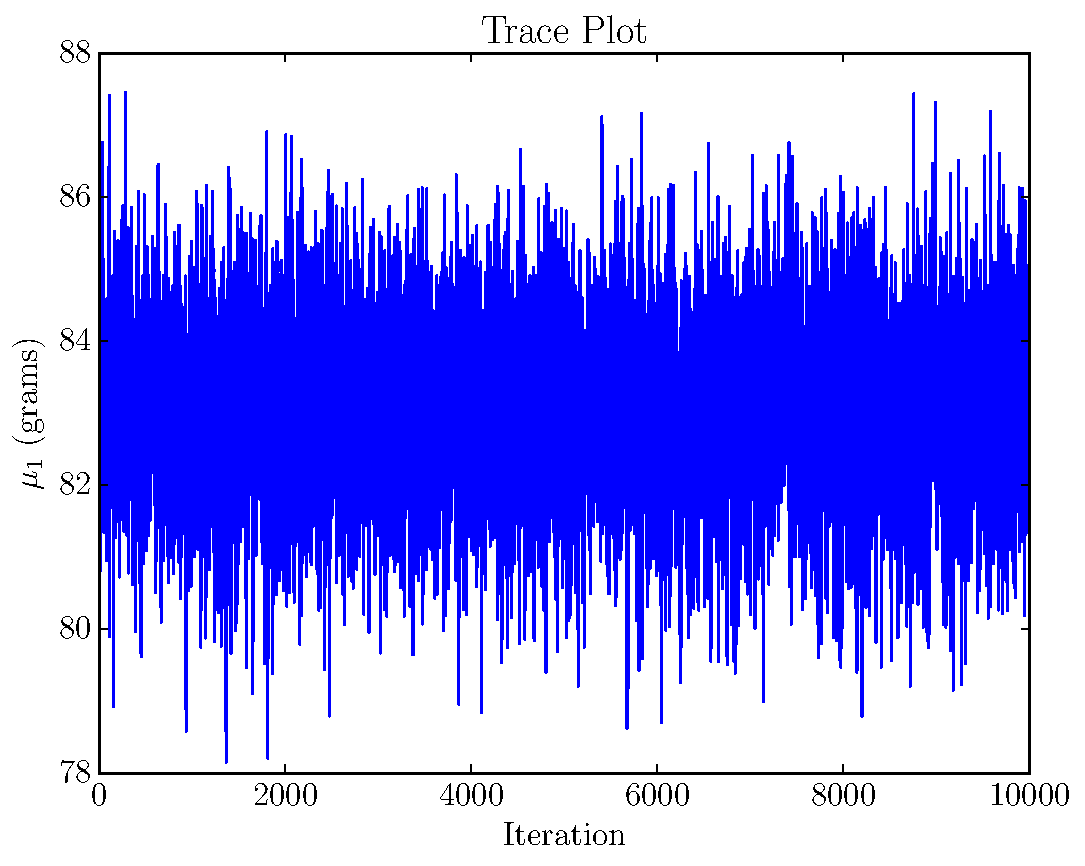
\includegraphics[scale=0.6]{Figures/trace_starlings2.pdf}
\end{center}
\end{figure}

